\documentclass{anstrans}
%%%%%%%%%%%%%%%%%%%%%%%%%%%%%%%%%%%
\title{Implementation of the SP3 equations in a MOOSE-based application}
\author{Roberto E. Fairhurst Agosta, Kathryn D. Huff}

\institute{
University of Illinois at Urbana-Champaign, Dept. of Nuclear, Plasma, and Radiological Engineering\\
ref3@illinois.edu
}

%%%% packages and definitions (optional)
\usepackage{graphicx} % allows inclusion of graphics
\usepackage{booktabs} % nice rules (thick lines) for tables
\usepackage{microtype} % improves typography for PDF
\usepackage{xspace}
\usepackage{tabularx}
\usepackage{floatrow}
\usepackage{subcaption}
\usepackage{enumitem}
\usepackage{placeins}
\usepackage{amsmath}
\usepackage[acronym,toc]{glossaries}
\newacronym{ANL}{ANL}{Argonne National Laboratory}
\newacronym{API}{API}{Application Programming Interface}
\newacronym{B4C}{B4C}{boron carbide}
\newacronym{BC}{BC}{boundary condition}
\newacronym{BOC}{BOC}{beginning of the equilibrium cycle}
\newacronym{BSD}{BSD}{Berkeley Software Distribution}
\newacronym{BWR}{BWR}{Boiling Water Reactor}
\newacronym{CAISO}{CAISO}{California ISO}
\newacronym{CAPP}{CAPP}{Core Analyzer for Pebble and Prism type VHTRs}
\newacronym{CEA}{CEA}{Commissariat a l'Energie Atomique}
\newacronym{CFD}{CFD}{computational fluid dynamics}
\newacronym{CO2}{CO$_2$}{carbon dioxide}
\newacronym{CR}{CR}{control rod}
\newacronym{CRP}{CRP}{Coordinated Research Project}
\newacronym{CZP}{CZP}{Cold Zero Power}
\newacronym{DCC}{DCC}{depressurized conduction cool-down}
\newacronym{DOE}{DOE}{Department of Energy}
\newacronym[\glslongpluralkey={degrees of freedom}]{DoF}{DoF}{degree of freedom}
\newacronym{EOC}{EOEC}{end of the equilibrium cycle}
\newacronym{FCEV}{FCEV}{Fuel Cell Electric Vehicle}
\newacronym{FDM}{FDM}{Finite Difference Method}
\newacronym{FEM}{FEM}{Finite Element Method}
\newacronym{FVM}{FVM}{Finite Volume Method}
\newacronym[\glslongpluralkey={greenhouse gases}]{GHG}{GHG}{greenhouse gas}
\newacronym{GRS}{GRS}{Gesellschaft für Anlagen und Reaktorsicherheit}
\newacronym{GT-MHR}{GT-MHR}{Gas Turbine-Modular Helium Reactor}
\newacronym{H2}{H$_2$}{hydrogen}
\newacronym{He}{He}{helium}
\newacronym{HFP}{HFP}{Hot Full Power}
\newacronym{HPCC}{HPCC}{high-pressure conduction cool-down}
\newacronym{HTE}{HTE}{High-Temperature Electrolysis}
\newacronym{HTGR}{HTGR}{High-Temperature Gas-Cooled Reactor}
\newacronym{HTR}{HTR}{High Temperature Reactor}
\newacronym{HTTR}{HTTR}{High-Temperature engineering Test Reactor}
\newacronym{HZDR}{HZDR}{Helmholtz-Zentrum Dresden-Rossendorf}
\newacronym{IAEA}{IAEA}{International Atomic Energy Agency}
\newacronym{icap}{iCAP}{Illinois Climate Action Plan}
\newacronym{INL}{INL}{Idaho National Laboratory}
\newacronym{IPyC}{IPyC}{inner pyrolytic carbon}
\newacronym{JFNK}{JFNK}{Jacobian-Free Newton-Krylov}
\newacronym{KAERI}{KAERI}{Korea Atomic Energy Research Institute}
\newacronym{Keff}{k$_{eff}$}{multiplication factor}
\newacronym{LBP}{LBP}{Lumped Burnable Poison}
\newacronym{LGPL}{LGPL}{Lesser GNU Public License}
\newacronym{LOCA}{LOCA}{loss of coolant accident}
\newacronym{LPCC}{LPCC}{low-pressure conduction cool-down}
\newacronym{LTE}{LTE}{Low-Temperature Electrolysis}
\newacronym{LWR}{LWR}{Light Water Reactor}
\newacronym{MC}{MC}{Monte Carlo}
\newacronym{MHTGR}{MHTGR}{Modular High-Temperature Gas-Cooled Reactor}
\newacronym{MMR}{MMR}{Micro Modular Reactor}
\newacronym{MOC}{MOC}{middle of the equilibrium cycle}
\newacronym{MOX}{MOX}{mixed-oxide}
\newacronym{MOOSE}{MOOSE}{Multi-physics Object-Oriented Simulation Environment}
\newacronym{MPI}{MPI}{Message Passing Interface}
\newacronym{MSR}{MSR}{Molten Salt Reactor}
\newacronym{MTD}{MTD}{Champaign-Urbana Mass Transit District}
\newacronym{NEA}{NEA}{Nuclear Energy Agency}
\newacronym{NEM}{NEM}{Nodal Expansion Method}
\newacronym{NGNP}{NGNP}{Next Generation Nuclear Power}
\newacronym{NRC}{NRC}{Nuclear Regulatory Commission}
\newacronym{NSC}{NSC}{Nuclear Science Committee}
\newacronym{OECD}{OECD}{Organisation for Economic Co-operation and Development}
\newacronym{OPyC}{OPyC}{outer pyrolytic carbon}
\newacronym{ORNL}{ORNL}{Oak Ridge National Laboratory}
\newacronym{OS}{OS}{Operator-Splitting}
\newacronym{PBMR}{PBMR}{Pebble Bed Modular Reactor}
\newacronym{PDE}{PDE}{Partial Differential Equation}
\newacronym{PMR}{PMR}{Prismatic Modular Reactor}
\newacronym{PV}{PV}{photovoltaics}
\newacronym{RPV}{RPV}{Reactor Pressure Vessel}
\newacronym{RSC}{RSC}{Reserve Shutdown Control}
\newacronym{RSD}{RSD}{Relative Standard Deviation}
\newacronym{SD}{SD}{Standard Deviation}
\newacronym{SI}{SI}{Sulfur-Iodine}
\newacronym{SiC}{SiC}{silicon carbide}
\newacronym{SMR}{SMR}{Small Modular Reactor}
\newacronym{SNU}{SNU}{Seoul National University}
\newacronym{SOEC}{SOEC}{Solid Oxide Electrolysis Cells}
\newacronym{SP3}{SP$_3$}{Simplified P$_3$}
\newacronym{TIP}{TIP}{transverse integration procedure}
\newacronym{TRISO}{TRISO}{Tristructural Isotropic}
\newacronym{UIUC}{UIUC}{University of Illinois at Urbana-Champaign}
\newacronym{UNIST}{UNIST}{Ulsan National Institute of Science and Technology}
\newacronym{UK}{UK}{United Kingdom}
\newacronym{UMICH}{UMICH}{University of Michigan}
\newacronym{US}{US}{United States}
\newacronym{USNC}{USNC}{Ultra Safe Nuclear Corporation}
\newacronym{VHTR}{VHTR}{Very High-Temperature Gas-Cooled Reactor}
%\newacronym{<++>}{<++>}{<++>}
%\newacronym{<++>}{<++>}{<++>}

\makeglossaries

\usepackage[printwatermark]{xwatermark}
\usepackage{xcolor}
\usepackage{graphicx}
\usepackage{lipsum}

\newcommand{\SN}{S$_N$}
\renewcommand{\vec}[1]{\bm{#1}} %vector is bold italic
\newcommand{\vd}{\bm{\cdot}} % slightly bold vector dot
\newcommand{\grad}{\vec{\nabla}} % gradient
\newcommand{\ud}{\mathop{}\!\mathrm{d}} % upright derivative symbol

\newcolumntype{c}{>{\hsize=.56\hsize}X}
\newcolumntype{b}{>{\hsize=.7\hsize}X}
\newcolumntype{s}{>{\hsize=.74\hsize}X}
\newcolumntype{f}{>{\hsize=.1\hsize}X}
\newcolumntype{a}{>{\hsize=.45\hsize}X}
%\usepackage[pagestyles]{titlesec}
%\titleformat*{\subsection}{\normalfont}
%\titleformat{\section}{\bfseries}{Item \thesection.\ }{0pt}{}

%\newwatermark[allpages,color=gray!50,angle=45,scale=3,xpos=0,ypos=0]{DRAFT}

\begin{document}
%%%%%%%%%%%%%%%%%%%%%%%%%%%%%%%%%%%%%%%%%%%%%%%%%%%%%%%%%%%%%%%%%%%%%%%%%%%%%%%%

\section{Abstract}
% \textit{

% abstract goes here

% }

\section{Introduction}

% what am I doing


% MOOSE
MOOSE\cite{gaston_moose_2009} is a computational framework that supports engineering analysis applications.
In a nuclear reactor, several partial differential equations describe the physical behavior.
These equations are typically nonlinear, and they are often coupled to each other.
MOOSE targets such systems and solves them in a fully coupled manner.

MOOSE is an open-source \gls{FEM} framework.
The framework itself relies on LibMesh\cite{kirk_libmesh_2006} and PetSc\cite{balay_petsc_2016} for solving nonlinear equations.
MOOSE applications define weak forms of the governing equations and modularize the physics expressions into "kernels."
Kernels are C++ classes containing methods for computing the residual and Jacobian contributions of individual pieces of the governing equations.
MOOSE and LibMesh translate them into residual and Jacobian functions.
These functions become inputs into PetSc solution routines.

All the software built on the MOOSE framework shares the same \gls{API}, facilitating relatively easy coupling between different phenomena.
Additionally, the framework and its applications use \gls{MPI} for parallel communication and allow deployment on massively-parallel cluster-computing platforms.



% lit - review: the SPN approximation
The $P_N$ method \cite{davidson_neutron_1957} discretizes the transport equation by expanding the angular dependence of the neutron flux in spherical harmonics, considering up to order $N$ polynomials.
If $N \rightarrow \infty$, the solution of the $P_N$ equations tends to the exact transport solution.
In three-dimensional geometries, the number of $P_N$ equations is proportional to $(N+1)^2$, whereas, in one-dimensional planar geometries, the number of $P_N$ equations is $(N+1)$.
Gelbard \cite{gelbard_spherical_1960} proposed the $SP_N$ approximation by replacing the second derivatives in the one-dimensional planar $P_N$ equations with three-dimensional Laplacian operators.
This approximation considerably reduces the number of equations conserving a reasonable accuracy.


Although Gelbard proposed the $SP_N$ approximation in the 60s, the method did not have a strong theoretical basis until the 90s with Pomraning \cite{pomraning_asymptotic_1993}, Brantley, and Larsen's \cite{brantley_simplifiedP3_2000} contribution.


The disadvantage of the $SP_N$ approximation is that the solution does not usually converge to the true transport solution as $N \rightarrow \infty$.

The $SP_N$ equations yield asymptotic solutions of the transport equation in a physical regime in which diffusion theory is the leading-order approximation.



However, several results \cite{mui_modified_1987} \cite{beckert_development_2007} \cite{fliscounakis_potential_2012} \cite{ryu_finite_2013} \cite{khosravi_mirzaee_reactor_2019} show that the $SP_N$ approximation yields more accurate solutions than the diffusion approximation with considerably less computational expense than the discrete ordinates ($S_N$) method.


% why is SP3 preferred over diffusion



% lit - review: software using the SPN approximation
Currently, different software uses the SP3 approximation to solve the neutron transport equation, such as SCOPE2 \cite{tatsumi_object-oriented_2002}, PARCS \cite{downar_parcs_2004}, DYN3D \cite{beckert_development_2007}, SIMULATE-5 \cite{bahadir_studsviks_2009}, and COCAGNE \cite{fliscounakis_potential_2012}.




\section{Methodology}

% Equations P3
Davidson \cite{davidson_neutron_1957} defined the one dimensional multi-group P$_3$ equations 

\begin{align}
    & \frac{d}{dx} \phi_{1,g} + \Sigma_{t,g} \phi_{0,g} = \sum_{g'=1}^G \Sigma_{s0,g' \rightarrow g} \phi_{0,g'} + \frac{\chi_g}{k_{eff}} \sum_{g'=1}^G \nu\Sigma_{f,g'} \phi_{0,g'} \notag \\ & \quad \quad \quad \quad \quad \quad \quad + Q_{0,g}  \label{eq:P3-0} \\
    & \frac{1}{3} \frac{d}{dx} \phi_{0,g} + \frac{2}{3}\frac{d}{dx}\phi_{2,g} + \Sigma_{t,g} \phi_{1,g} = \sum_{g'=1}^G \Sigma_{s1,g' \rightarrow g} \phi_{1,g'} + Q_{1,g} \label{eq:P3-1} \\
    & \frac{2}{5} \frac{d}{dx}\phi_{1,g} + \frac{3}{5}\frac{d}{dx}\phi_{3,g} + \Sigma_{t,g} \phi_{2,g} = \sum_{g'=1}^G \Sigma_{s2,g' \rightarrow g} \phi_{2,g'} + Q_{2,g} \label{eq:P3-2} \\
    & \frac{3}{7}\frac{d}{dx}\phi_{2,g} + \Sigma_{t,g} \phi_{3,g} = \sum_{g'=1}^G \Sigma_{s3,g' \rightarrow g} \phi_{3,g'} + Q_{3,g} \label{eq:P3-3} \\
    \intertext{where}
    & \phi_{n,g} = \mbox{$n^{th}$ moment of group $g$ neutron flux}  \notag \\ %  } [n \cdot cm^{-2} \cdot s^{-1}]
    & \Sigma_{t,g} = \mbox{group $g$ macroscopic total cross-section}  \notag \\ %  } [cm^{-1}]
	& \Sigma_{sn,g' \rightarrow g} = \mbox{$n^{th}$ moment of the group $g'$ to group $g$} \notag \\
	& \mbox{macroscopic scattering cross-section}  \notag \\ %  } [cm^{-1}]
	& \nu\Sigma_{f,g} = \mbox{group $g$ macroscopic production cross-section}  \notag \\ %  } [cm^{-1}]
	& \chi_{g} = \mbox{group $g$ fission spectrum}  \notag \\ %  } [cm^{-1}]
	& k_{eff} = \mbox{multiplication factor}  \notag \\ %  } [-]
	& Q_{n,g} = \mbox{$n^{th}$ moment of group $g$ external neutron source}  \notag \\  % } [n \cdot cm^{-3} \cdot s^{-1}]
	& G = \mbox{number of energy groups}.  \notag % } [-]
\end{align}

Assuming an isotropic external source and a negligible anisotropic group-to-group scattering \cite{brantley_simplifiedP3_2000}
\begin{align}
	& Q_{n,g} = 0, \quad n > 0 \notag \\
	& \Sigma_{sn,g' \rightarrow g} = 0, \quad g' \ne g, \quad n > 0 \notag
\end{align}

\noindent
simplifies equations \ref{eq:P3-1} and \ref{eq:P3-3}, allowing to express the odd moments of the flux $\phi_{1,g}$ and $\phi_{3,g}$ as functions of the even moments $\phi_{0,g}$ and $\phi_{2,g}$.
Introducing $\phi_{1,g}$ and $\phi_{3,g}$ into equations \ref{eq:P3-0} and \ref{eq:P3-2} reduces the system of equations from four to two equations.
Introducing the variables $\Phi_{0,g}$ and $\Phi_{2,g}$, reorganizing the equations, and replacing the second derivatives by Laplacian operators \cite{gelbard_spherical_1960} yields the SP$_3$ equations

% Equations SP3
\begin{align}
    & - D_{0,g} \Delta \Phi_{0,g} + \Sigma_{0,g} \Phi_{0,g} - 2 \Sigma_{0,g} \Phi_{2,g} = S_{0,g} \label{eq:SP3-0e} \\
    & - D_{2,g} \Delta \Phi_{2,g} + \left( \Sigma_{2,g} + \frac{4}{5} \Sigma_{0,g} \right) \Phi_{2,g} - \frac{2}{5} \Sigma_{0,g} \Phi_{0,g} = -\frac{2}{5} S_{0,g}. \label{eq:SP3-2e}
    \intertext{where}
	& \Sigma_{n,g} = \Sigma_{t,g} - \Sigma_{sn,g' \rightarrow g} \notag \\
    & \Phi_{0,g} = \phi_{0,g} + 2 \phi_{2,g} \notag \\
    & \Phi_{2,g} = \phi_{2,g} \notag \\
    & D_{0,g} = \frac{1}{3 \Sigma_{1,g}} \notag \\
    & D_{2,g} = \frac{9}{35 \Sigma_{3,g}} \notag \\
    & S_{0,g} = \sum_{g'\ne g}^G \Sigma_{s0,g' \rightarrow g} \left( \Phi_{0,g'} - 2 \Phi_{2,g'} \right) \notag \\
    & \quad \quad + \frac{\chi_g}{k_{eff}} \sum_{g'=1}^G \nu\Sigma_{f,g'} \left( \Phi_{0,g'} - 2 \Phi_{2,g'} \right) + Q_{0,g}. \notag
\end{align}

% BCs
The Marshak-like vacuum \glspl{BC} complete the system of equations \cite{beckert_development_2007}

\begin{align}
    & \frac{1}{4} \Phi_{0,g} \pm \frac{1}{2} \hat{n} \cdot J_{0,g} - \frac{3}{16} \Phi_{2,g} = 0 \label{eq:SP3-BC1a} \\
    - & \frac{3}{80} \Phi_{0,g} \pm \frac{1}{2} \hat{n} \cdot J_{2,g} + \frac{21}{80} \Phi_{2,g} = 0 \label{eq:SP3-BC2a}
    \intertext{where}
    & J_{n,g} = -D_{n,g} \nabla \Phi_{n,g}. \notag
\end{align}

\section{Results}

\subsection{C5 MOX Benchmark}

% intro to the benchmark
OECD/NEACRP-L-336 C5 MOX fuel benchmark \cite{cavarec_benchmark_1994}

The \gls{OECD}/\gls{NEA} developed this benchmark to carry out validation of methods and identify their strengths, limitations, and accuracy, and to suggest needs for method development.

The definition of the original benchmark can be found in .

% why is SP3 preferred over diffusion: maybe move to intro ??
MOX fuel assemblies have higher thermal absorption and fission cross-sections than UO$_2$ fuel assemblies.
Consequently, the thermal flux is lower while the power production higher.
Modeling these characteristics of reactors using MOX fuel using the diffusion approximation may be challenging.

% benchmark specification
Two types of fuel assembly (MOX and UO$_2$) and a reflector comprise the core, shown in Figure \ref{fig:bench1}.
Due to the problem's symmetry, the model included only a quarter of the core.
Each fuel assembly consists of a 17 $\times$ 17 array of squared pin cells, as displayed in Figures \ref{fig:bench2} and \ref{fig:bench3}.
The dimensions of each pin cell are 1.26 $\times$ 1.26 cm, being 21.42 $\times$ 21.42 cm the length of each assembly, and 128.52 $\times$ 128.52 cm.

The benchmark \cite{cavarec_benchmark_1994} specifies the cross-sections, which have a two-energy group structure.

% add reference
Gmsh

\begin{figure}[htbp!] %or H 
    \centering
    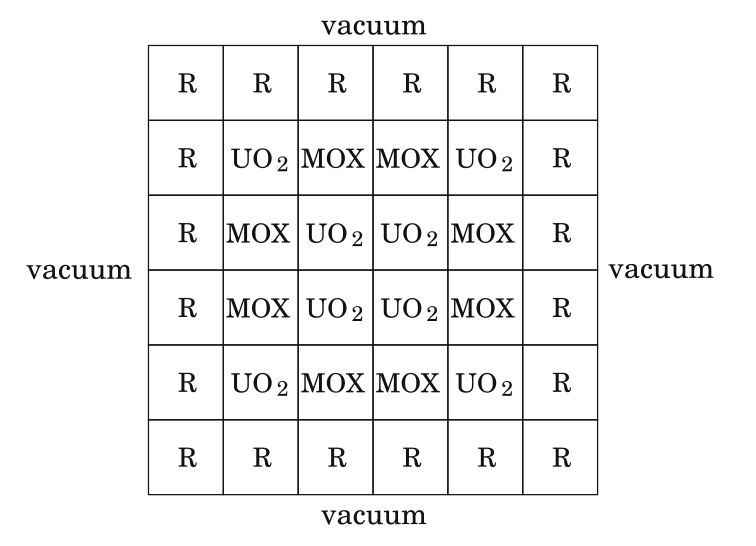
\includegraphics[width=0.95\linewidth]{figures/bench-config.png}
    \hfill
    \caption{C5 MOX benchmark configuration. \textit{R} correponds to the reflector region. Image reproduced from \cite{capilla_applications_2009}.}
    \label{fig:bench1}
\end{figure}

\begin{figure}[htbp!] %or H 
    \centering
    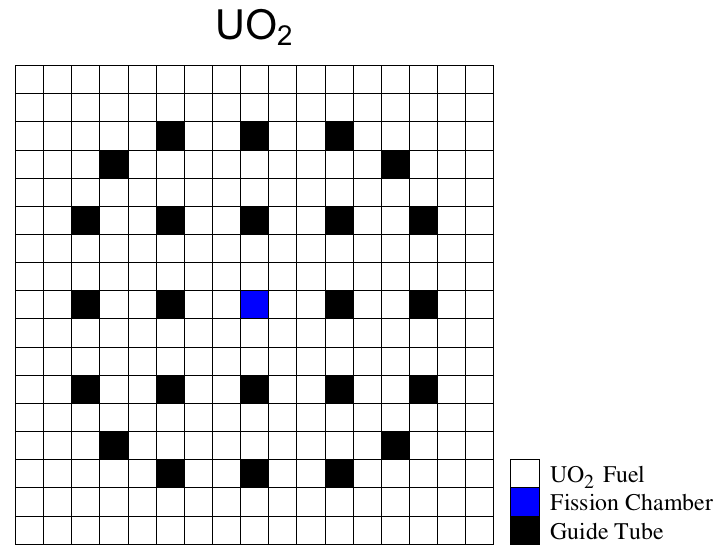
\includegraphics[width=0.95\linewidth]{figures/bench-config2.png}
    \hfill
    \caption{Structure of the UO$_2$ assembly. Image reproduced from \cite{capilla_applications_2009}.}
    \label{fig:bench2}
\end{figure}

\begin{figure}[htbp!] %or H 
    \centering
    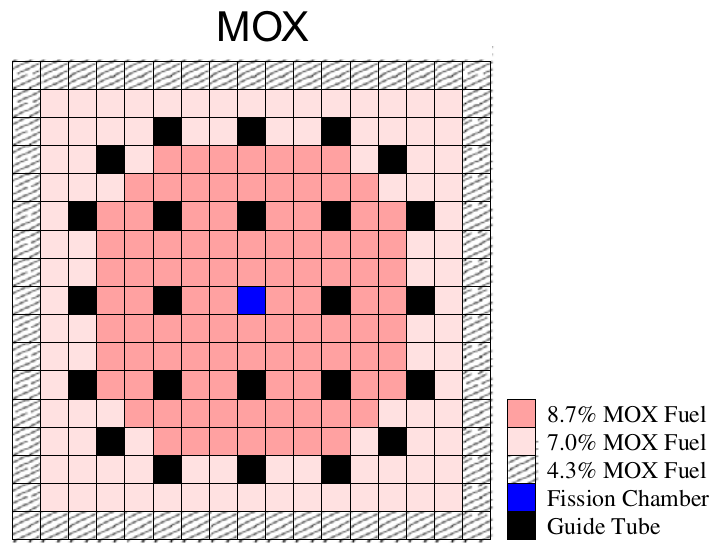
\includegraphics[width=0.95\linewidth]{figures/bench-config3.png}
    \hfill
    \caption{Structure of the MOX assembly. Image reproduced from \cite{capilla_applications_2009}.}
    \label{fig:bench3}
\end{figure}

Normal \cite{capilla_applications_2009}
Diagonal transport correction \cite{cavarec_benchmark_1994}

% \usepackage{booktabs}
\begin{table}[]
	\centering
	\caption{\gls{GGE}, \gls{DGE}, and CO$_2$ produced.}
	\label{tab:meth}
	\begin{tabular}{llll}
	\toprule
							& Reference & MOOSE & $\Delta_{\rho}$ 	\\
	\midrule
	Normal 					&			&		&					\\
	Transport correction 	&			&		&					\\
	\bottomrule
	\end{tabular}
\end{table}

% Discussion ?

Diagonal transport correction:
C5 MOX Benchmark \cite{cavarec_benchmark_1994}, PARCS \cite{downar_parcs_2004}, DYN3D \cite{beckert_development_2007}

\section{Conclusions}



\section{Acknowledgements}

% Not sure about this
Roberto E. Fairhurst Agosta and Prof. Huff are supported by the \gls{NRC} Faculty Development Program (award NRC-HQ-84-14-G-0054 Program B).
Prof. Huff is also supported by the Blue Waters sustained-petascale computing project supported by the National Science Foundation (awards OCI-0725070 and ACI-1238993) and the state of Illinois, the DOE ARPA-E MEITNER Program (award DE-AR0000983), the DOE H2@Scale Program (award), and the International Institute for Carbon Neutral Energy Research (WPI-I2CNER), sponsored by the Japanese Ministry of Education, Culture, Sports, Science and Technology.

%%%%%%%%%%%%%%%%%%%%%%%%%%%%%%%%%%%%%%%%%%%%%%%%%%%%%%%%%%%%%%%%%%%%%%%%%%%%%%%%
\bibliographystyle{ans}
\bibliography{bibliography}
\end{document}

% \begin{figure}[htbp!] %or H 
%     \centering
%     \includegraphics[width=0.95\linewidth]{figures/radial-layout.png}
%     \hfill
%     \caption{Core radial layout. Image reproduced from \cite{oecd_nea_benchmark_2017}.}
%     \label{fig:radial}
% \end{figure}

% \begin{align}
%     \frac{1}{v_g}\frac{\partial}{\partial t} \phi_g &= \nabla \cdot D_g
%     \nabla \phi_g - \Sigma_g^r \phi_g \sum_{g \ne g'}^G
%     \Sigma_{g'\rightarrow g}^s \phi_{g'} \label{eq:diffusion}
%     \intertext{where}
%     C_i &= \mbox{concentration of delayed neutron precursors} \notag \\
%     &\phantom{{}=1} \mbox{in precursor group $i$}.
% \end{align}
